\centering

\tikzstyle{state} = [circle,thick,minimum size=1.2cm,draw=black]
\tikzstyle{assoc} = [circle,thick,minimum size=1.2cm,draw=blue]
\tikzstyle{exist} = [circle,thick,minimum size=1.2cm,draw=green]
\tikzstyle{observ} = [circle,thick,minimum size=1.2cm,draw=red]


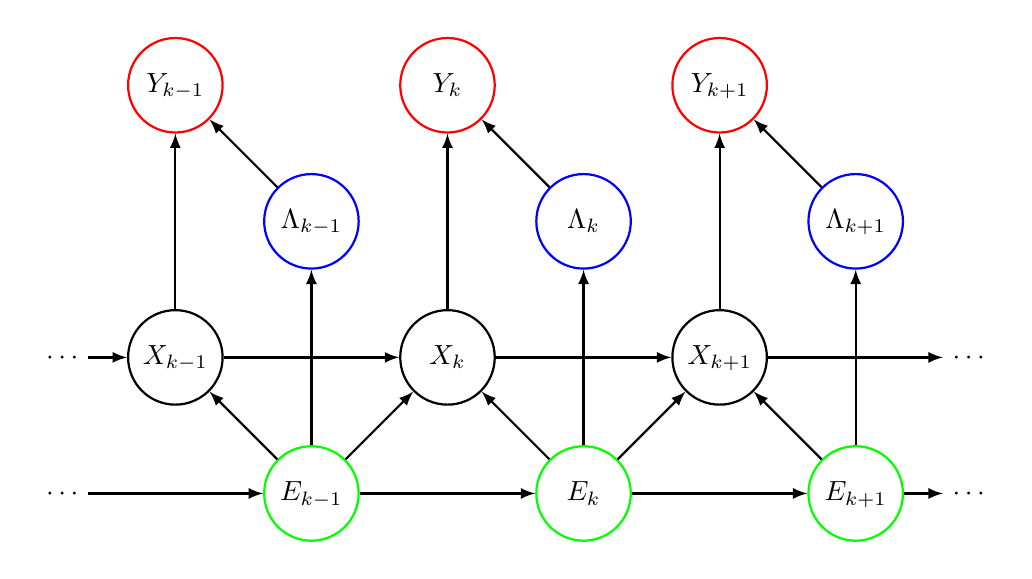
\begin{tikzpicture}[>=latex,text height=1.5ex,text depth=0.25ex]

	\matrix[row sep=0.5cm,column sep=0.5cm] {
		&
		\node (y_k-1) [observ]{$Y_{k-1}$}; &
		&
		\node (y_k) [observ]{$Y_{k}$}; &
		&
		\node (y_k+1) [observ]{$Y_{k+1}$}; &
		& \\
		& &
		\node (l_k-1) [assoc]{$\Lambda_{k-1}$}; &
		&
		\node (l_k) [assoc]{$\Lambda_{k}$}; &
		&
		\node (l_k+1) [assoc]{$\Lambda_{k+1}$}; & \\
		\node (x_k-2) {$\cdots$}; &
		\node (x_k-1) [state]{$X_{k-1}$}; &
		&
		\node (x_k) [state]{$X_{k}$}; &
		&
		\node (x_k+1) [state]{$X_{k+1}$}; &
		&
		\node (x_k+2) {$\cdots$}; \\
		\node (e_k-2) {$\cdots$}; & &
		\node (e_k-1) [exist]{$E_{k-1}$}; &
		&
		\node (e_k) [exist]{$E_{k}$}; &
		&
		\node (e_k+1) [exist]{$E_{k+1}$}; &
		\node (e_k+2) {$\cdots$}; \\
	};

	\path[->]
		(x_k-2) edge[thick] (x_k-1)
		(x_k-1) edge[thick] (x_k)
		(x_k) edge[thick] (x_k+1)
		(x_k+1) edge[thick] (x_k+2)
		
		(x_k-1) edge[thick] (y_k-1)
		(x_k) edge[thick] (y_k)
		(x_k+1) edge[thick] (y_k+1)
		
		(l_k-1) edge[thick] (y_k-1)
		(l_k) edge[thick] (y_k)
		(l_k+1) edge[thick] (y_k+1)
		
		(e_k-2) edge[thick] (e_k-1)
		(e_k-1) edge[thick] (e_k)
		(e_k) edge[thick] (e_k+1)
		(e_k+1) edge[thick] (e_k+2)
		
		(e_k-1) edge[thick] (x_k-1)
		(e_k) edge[thick] (x_k)
		(e_k+1) edge[thick] (x_k+1)
		
		(e_k-1) edge[thick] (x_k)
		(e_k) edge[thick] (x_k+1)
		
		(e_k-1) edge[thick] (l_k-1)
		(e_k) edge[thick] (l_k)
		(e_k+1) edge[thick] (l_k+1)
		;

\end{tikzpicture}